\documentclass{article}
\usepackage{graphicx}
\usepackage{hyperref}
\usepackage{algorithm}
\usepackage{algpseudocode}
\usepackage[
    top=0.5in,
    bottom=0.9in,
    left=0.75in,
    right=0.75in
]{geometry}

\title{\textbf{GPU Computing} \\
    \large Homework 1: Matrix Transposition \\
}
\author{Murtas Cristian \\ 248025 \\ cristian.murtas@studenti.unitn.it \\
\href{https://github.com/SecondarySkyler/gpu-computing/tree/main/matrix_transposition}{GitHub Repository}
} 

\begin{document}
\maketitle

\section{Problem Description}
The goal of this homework is to implement a matrix transposition algorithm, where the transpose of a matrix
is an operator which flips the matrix over its diagonal. That is, if $A$ is a matrix of size $m \times n$, then
the transpose of $A$ is a matrix of size $n \times m$ where the element at row $i$ and column $j$ is the element,
also denoted as $A\textsuperscript{T}$. \\
Additionally, we are asked to measure the effective bandwidth of our implementation, considering also the
usage of different optimization flags such as: \texttt{-O0}, \texttt{-O1}, \texttt{-O2}, \texttt{-O3}. \\
Furthermore an analysis of the cache behavior of the algorithm is required, for this purpose we are going to use
valgrind.
\subsection{Algorithm}
In order to dimostrare qualcosa, two algorithms have been implemented: the first one is a na\"{i}ve approach, which
consists in iterating over the matrix and swapping the elements, while the second one is a more optimized version
which takes advantage of a block mechanism to reduce the number of cache misses.
\begin{algorithm}
    \caption{Na\"{i}ve Matrix Transposition}
    \begin{algorithmic}[1]
        \State $src \gets create\_matrix(size)$
        \For{$i = 0$ to $size$}
            \For{$j = 0$ to $size$}
                \State $dest[j * size + i] = src[i * size + j]$
            \EndFor
        \EndFor
    \end{algorithmic}
\end{algorithm}

\section{Bo da decidere}
\subsection{Hardware}
\begin{enumerate}
    \item \textbf{Desktop PC}
    \begin{itemize}
        \item \textbf{CPU}: AMD Ryzen 5 5600X
        \begin{itemize}
            \item \textbf{Cores}: 6
            \item \textbf{Threads}: 12
            \item \textbf{Base Clock}: 3.7 GHz
            \item \textbf{L1 Cache}: 64 KB (per core)
            \item \textbf{L2 Cache}: 512 KB (per core)
            \item \textbf{L3 Cache}: 32 MB
        \end{itemize}
        \item \textbf{RAM}: 16 GB DDR4
        \item \textbf{OS}: Ubuntu 22.04 (on WSL2)
    \end{itemize}
    \item \textbf{MacBook Air M1}
    \begin{itemize}
        \item \textbf{CPU}: Apple M1
        \begin{itemize}
            \item \textbf{Cores}: 8 (4 Firestorm + 4 Icestorm)
            \item \textbf{Threads}: 8
            \item \textbf{Base Clock}: 3.2 GHz
            \item \textbf{L1 Cache Firestorm}: 192 + 128 KB (instructions + data, per core)
            \item \textbf{L2 Cache Firestorm}: 12 MB (shared)
            \item \textbf{L1 Cache Icestorm}: 128 + 64 KB (instructions + data, per core)
            \item \textbf{L2 Cache Icestorm}: 4 MB (shared)
        \end{itemize}
        \item \textbf{RAM}: 8 GB LPDDR4X
        \item \textbf{OS}: macOS Ventura 13.2.1
    \end{itemize}
\end{enumerate}
\subsection{Results}
\begin{figure}[H]
    \centering
    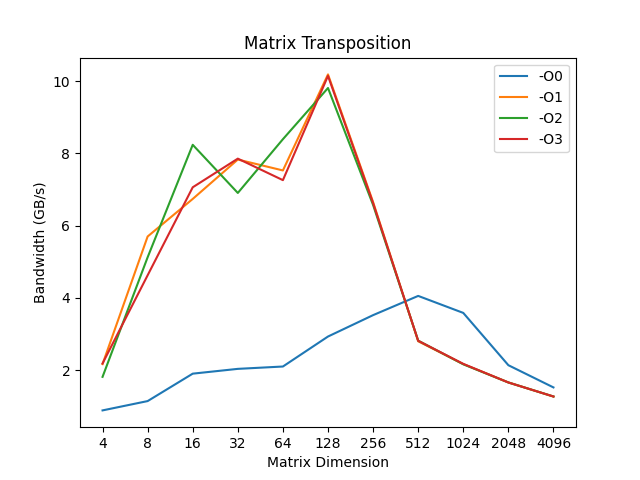
\includegraphics[]{report/img/output.png}
    \caption{}
\end{figure}
\section{Conclusion}
\end{document}

